\section{Internet of Plants}

\subsection{Overview}

The Internet of Plants, also called IoP, is a concept that aims to interconnect the plant device previously built.
This in order to empower the device capabilities and to provide a better user experience.
This project includes:
\begin{itemize}
    \item A better sound quality by using professional sonification software
    \item The ability to create a full artistic experience by creating a distributed instrument
    \item Refining the interaction with the plant by using more complex data analyses
\end{itemize}



\subsection{Communication}

On the communication side, we benchmarked several communication protocol including internet protocol,
Bluetooth, Bluetooth Low Energy and Zigbee (ref to table \ref{tab:protocol_comparison}).

\begin{table}[]
    \begin{tabular}{|l|l|l|l|l|}
        \hline
        Protocol                            & IP   & Bluetooth & BLE   & Zigbee \\ \hline
        Handle multiple connections         & Yes  & No        & No    & Yes    \\
        Requires additional hardware        & No   & No        & No    & Yes    \\
        Subject to interference             & Yes  & Few       & Few   & Yes    \\
        Energy efficiency (using a battery) & Days & Months    & Years & Years  \\ \hline
    \end{tabular}
    \caption{Comparison between different communication protocol to find the one that will suits our needs.}
    \label{tab:protocol_comparison}
\end{table}

The IP protocol (whether it is on WiFi or Ethernet) has been chosen for this application for several reasons:

\begin{itemize}
    \item \textbf{High bandwidth}: It supports the transmission of large amounts of data quickly and efficiently, which is essential for real-time interactions in the system.
    \item \textbf{Widespread availability}: WiFi and Ethernet are commonly available in most exhibition spaces, ensuring easy deployment in a variety of environments.
    \item \textbf{Multi-device connectivity}: The protocol allows the connection of multiple devices simultaneously, which is crucial for building a distributed system where many plants can interact with the server.
    \item \textbf{Compatibility}: Ethernet is already available on the server, and WiFi is built into the ESP32, eliminating the need for additional hardware.
\end{itemize}

The communication system is based on WiFi technology, leveraging the ESP32's built-in wireless capabilities. Both the server and the ESP32 devices are connected to the same local network. Data is transmitted from the ESP32 to the server using the IP protocol via a TCP (Transmission Control Protocol) socket. Each ESP32 opens a dedicated TCP socket to the server, and the server is capable of handling multiple sockets simultaneously—one for each connected device. The server is connected to the local network via an Ethernet cable, providing a stable, high-speed connection for data processing and sonification (ref figure \ref{fig:network_architecture}).

\begin{figure}[h]
    \centering
    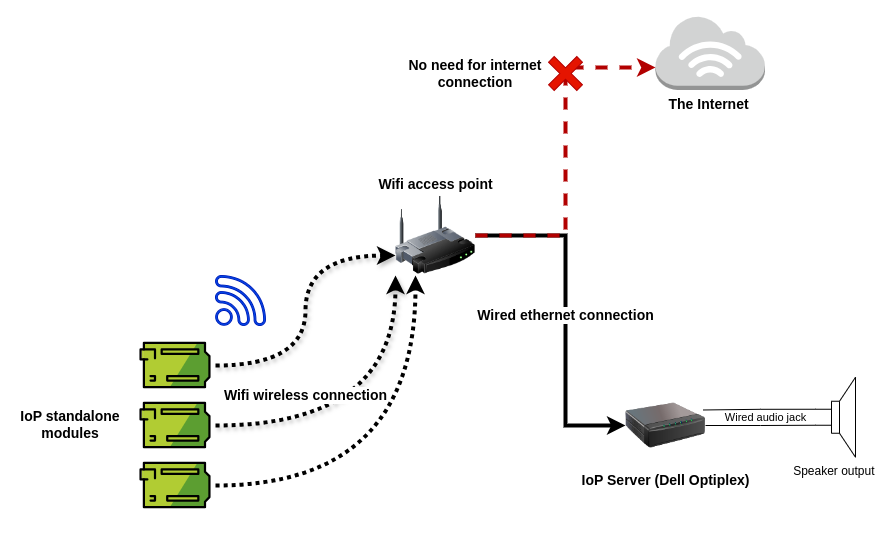
\includegraphics[width=\textwidth]{network_architecture.png}
    \caption{Schematic of the network architecture of the Internet of Plants project. The standalone modules are connected to the server using WiFi. The server is connected via Ethernet cable to the local access point. The server is also connected to a jack speaker working as output.}
    \vspace{0.1cm}
    \label{fig:network_architecture}
\end{figure}

However, a potential drawback of using IP networks is that they can become overcrowded, especially in environments with high network traffic, which may lead to packet loss or truncated data frames. To mitigate these issues, a start ("#") and stop (";\\n") character is embedded in the data transmission protocol. This structure helps the server recognize the beginning and end of each message, allowing it to discard incomplete or corrupted frames and process only complete, intact data. This approach minimizes the impact of network congestion by ensuring that even if a frame is truncated or lost, the server can still recover and process the next full message without error.

Additionally, this strategy helps maintain a balance within the CAP theorem (Consistency, Availability, and Partition tolerance). While it is impossible to achieve all three properties perfectly in a distributed system, the chosen protocol structure ensures data consistency by filtering out incomplete messages, availability by maintaining active connections across multiple devices, and some degree of partition tolerance in the event of temporary network failures. This balance is critical for ensuring reliable data transmission and processing in the Internet of Plants system.





\subsection{Server}

The server is a small fanless computer (Dell Optiplex) running Lubuntu. Lubuntu is a lighter version of Ubuntu that includes LXQt as desktop environnement. The choice of a distribution with graphical interface is induced by the use of \textit{Pure Data} as sonification software. However, the server can be run without graphical interface when on production mode. The choice of the light desktop environment is induced by the fact that the server is a low resources computer. The server only include 1 GB of RAM which is a limitation. The server is connected to the local network using an Ethernet cable. The server is also connected to a jack speaker (ref figure \ref{fig:network_architecture}).




%TODO: Add a picture of the  real setup

\textit{Pure Data} (PD) is an open-source visual programming language designed primarily for creating interactive multimedia applications, particularly in the fields of audio, video, and graphical processing.
\textit{Pure Data} is part of a family of patcher programming languages, which also includes Max/MSP.
Unlike traditional text-based programming, PD uses a graphical interface where users connect
"objects" with virtual patch cables to create complex data flows and signal processing chains.
Its modular design allows for real-time manipulation of sound and graphics, making it a powerful
tool for artists, musicians, and researchers interested in exploring experimental media.

\textit{Pure Data} requires, in a development environnement, a graphical interface to test and debug.
The \textit{Pure Data} patch receive the data through a TCP socket. The data is processed through several
operations. Then, if a threshold is passed, an interaction happened and the music is triggered.
The music is outputted through the item \textit{DAC} which means Digital to Analog Converter.
The digital input from \textit{Pure Data} is converted to a sound that speakers can output.

\begin{figure}[h]
    \centering
    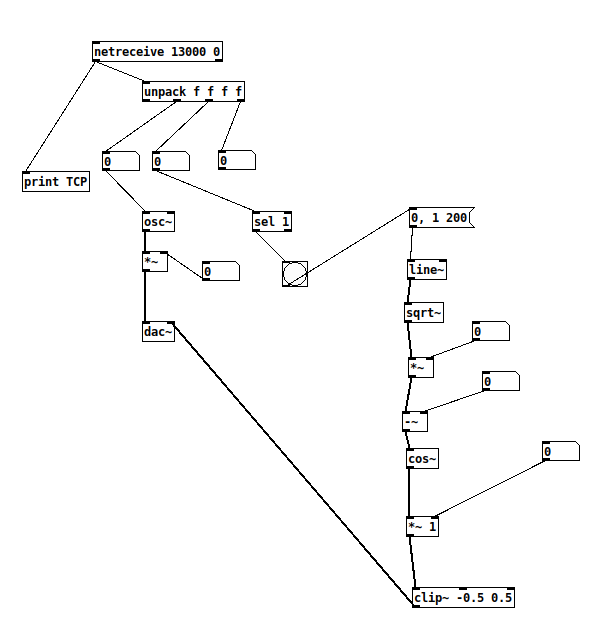
\includegraphics[width=\textwidth]{pure_data_patch.png}
    \caption{Basic \textit{Pure Data} patch that is used for sonification of the data
        of the plant. In case of an art exhibition, the \textit{Pure Data} patch can be upgraded to meet the
        artist needs}
    \vspace{0.1cm}
    \label{fig:pure_data_patch}
\end{figure}


\textit{Pure Data} is a sonification software that require data as input. In order to get and process the data, we designed a Python based software. %FIXME: microservices
The software is object oriented. The standalone IoP modules connect using WiFi to the receiver module
of the software. The connection is made using TCP socket from the ESP32 to the server.
The main module of the software then creates software abstraction of the standalone module.
The abstraction module is processing and storing all the processed data.
The main module then send the processed data to \textit{Pure Data} patch using also local TCP socket.

\begin{figure}[h]
    \centering
    \includegraphics[width=\textwidth]{iop_architecture.png}
    \caption{Architecture diagram of Internet of Plants project centered on server-side.}
    \vspace{0.1cm}
    \label{fig:server_architecture}
\end{figure}


\subsection{Deployment} %and application}

The server software is easily deployable. The software includes a shell script to deploy the server service (ref figure \ref{fig:install_script_logic}).
Indeed, the server relies on a \textit{systemd} linux service. \textit{Systemd} \cite{Both2020} is a Linux software that manage application that runs \textit{daemons} or services.
\textit{Daemons} are pieces of software that run in background of the operating
system. They are mainly started at the during the boot of the operating system.

\begin{figure}[h!]
    \centering
    \includegraphics[width=0.8\textwidth]{install_script_logic.png}
    \caption{Logic of the installation script. The script install the Python dependencies, fill in the templated service file, install the service and enable it.}
    \vspace{0.1cm}
    \label{fig:install_script_logic}
\end{figure}

The server is deployed using systemd service to allow the software to start with the operating system.
It waits for the network interfaces to be up and running and opens the socket.
The installation tool install Python dependencies, fill in the templated service file,
install the service and enable it. The server is able to receive data from IoP standalone
modules and use \textit{Pure Data} software for sonification. The last step is to connect
a jack speaker to the jack builtin output.

On the IoP standalone module side, it requires a software that is able to upload
firmware to an ESP32 MCU. I recommend using PlatformIO which is an open source
embedded software development platform. The firmware is developed using this platform.
The source code is written in C++ using the Arduino framework. You flash the firmware
to the chip after setting up the WiFi credentials.
The module sends all the retrieved data to the server.

\subsubsection{Distributed instruments}

The Internet of Plants (IoP) architecture enables the creation of a distributed instrument, where multiple IoP standalone modules can be deployed across different plants to form an interconnected musical system. Each module, linked to the server via WiFi, sends data collected from plant interactions, which the server then processes. By assigning unique IDs to each module, the server can differentiate between the various plants, allowing for distinct musical outputs based on the origin of the data.

The system sends this data to \textit{Pure Data} (PD), an open-source visual programming language for multimedia applications, where sound parameters such as pitch, tone, and rhythm can be finely controlled. This setup allows for highly customizable soundscapes, where each plant generates unique sounds based on user interaction, creating a rich, immersive musical experience. The distributed instrument thus transforms the interaction with plants into a collaborative musical performance, opening up new possibilities for art installations and interactive environments.

\subsection{output}

\subsubsection{Evauation}

%TODO: Create a Table that regroup frame dropped vs frame received
%TODO: Create a table 

\subsubsection{Art exhibition}

To push further the distributed instrument, it is possible to build an entire
musical experience for an art exhibition.
The immersive experience can take place as a fully connected forest. The music would vary
depending on the touch interaction that people have with the plants.

\begin{figure}[h!]
    \centering
    \includegraphics[width=\textwidth]{art_exhibition.pdf}
    \caption{Schematic of the IoP art exhibition. The music varies depending on the
        interaction that people have with the installation. People are immersed into the full
        musical and sonification experience.}
    \vspace{0.1cm}
    \label{fig:art_exhibition}
\end{figure}

This exhibition could allow people to rethink the way the see and interact with plants.
Plants are not seen anymore as decoration object but as a living being.
The living being is here highlighted by the fact that plants can now express their state.
The humidity level, the light intensity and other state signs are modifying the plant
reaction.


Musicians can also work in pair with plants to create songs using music from the plants.
The music coming from the plant is fully configurable with the sonification software.


\subsubsection{Final product, limitations and future work}

Final product is a software that allows the connection between multiple standalone IoP modules and a sonification software, \textit{Pure Data}. The software handle multiple connection and apply a filtering and cleaning on the data
retrieved. The data is then sent to \textit{Pure Data} for sonification.

As a demo and in order to do a photo shooting, we built up a system using the standalone module, connected through wire (ref figure \ref{fig:standalone_demo}). We used the serial communication in this demo because we did not have wireless communication usable at the shooting site. The computer is showing a visualization from the incoming data. This is a waterwall like visualization (ref figure \ref{fig:extracted_frame_demo}). The data is processed and displayed on the computer screen. The data is normalized on the y-axis. The x-axis is the sweep frequency. The graph signal at the bottom is the real-time signal. The computer is also producing the sound using \textit{Pure Data} software.

\begin{figure}[h!]
    \centering
    \includegraphics[width=0.8\textwidth]{server_module_demo.jpg}
    \caption{Server-module demo. In this specific use case, the module is connected by wire to a computer. Otherwise, the module is usable wirelessly.The computer is acting as a server. On this version of the demo, the screen is displaying a figure that is evolving depending on the touch interaction. The computer, acting as the server, is producing the sound using \textit{Pure Data} software.}
    \vspace{0.1cm}
    \label{fig:server_module_demo}
\end{figure}

\begin{figure}[h!]
    \centering
    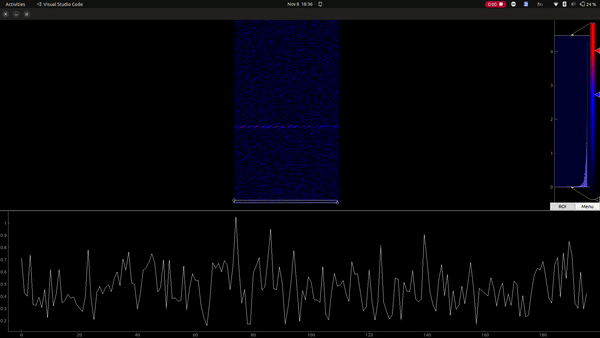
\includegraphics[width=\textwidth]{extracted_frame_demo.png}
    \caption{Waterfall like visualization of the data extracted from the standalone module. The data is processed and displayed on the computer screen. The data is normalized on the y-axis. The x-axis is the sweep frequency. The graph signal at the bottom is the real-time signal.}
    \vspace{0.1cm}
    \label{fig:extracted_frame_demo}
\end{figure}

On the limitation side, the use of WiFi ease a lot the deployment of the system, however
% Talk about a better fault tolerant way of communicating.
% About monitoring
% TODO: Talk about overcrowded wifi
% talk about frame dropped and lost. 
% Talk about the start and stop tag to check if frame is entire

\subsection{Conclusion}

In conclusion, the Internet of Plants (IoP) is a revolutionary application of IoT principles to plant systems, enabling more sophisticated interaction between humans and plants. By leveraging distributed systems, sensors, and sonification software, the IoP creates immersive environments where plants can become interactive instruments, generating real-time musical responses based on human touch. This innovation extends beyond artistic installations, providing new opportunities in agriculture, environmental monitoring, and human-computer interaction. However, limitations such as network congestion, sensor accuracy, and audio quality need further work to fully unlock the potential of plant-based sensor networks.

